\chapter{Wishbone Interconnect Overview}
\label{APP_Wishbone}

\section{Wishbone Interconnect Introduction}
Wishbone was designed as an internal interconnection standard for
System-on-a-Chip (Soc) applications (see www.OpenCores.org, the current home of
Wishbone project, and the contains the full specification). Wishbone is an
intended as a solution to provide a standard interface for communicating
between logic cores from multiple vendors. It can be difficult to
integrate logic cores if they each use a different interconnect scheme, and
this can also add significant overhead (logic and latency).

\subsection{Features}
The Wishbone design was inspired by traditional microcomputer
buses\cite{WB3_Spec}, like PCI and VME, as these are general purpose
interconnects that are flexible and robust.

A brief summary of important Wishbone features:
\begin{itemize}
  \item Supports reads and writes, burst and single-word transfers.
  \item Simple, logic resource requirements are low. At its simplest, an
  interface to a synchronous SRAM requires just one logic gate.
  \item User-defined tags allows the addition of extra signals.
  \item Support for data bit-widths of 8, 16, 32, and 64.
  \item Any address bit-width is supported, even zero, depending on the device.
  \item Synchronous; all transfers occur on clock edges.
  \item Choice of topology, i.e. bus, point-to-point, crossbar switch, is up to
  the system designer.
  \item Not encumbered by patents, free for all to use.
  \item A single device can be both a master and a slave.
  \item Offers some support for handling errors.
\end{itemize}


\subsection{A Simple Example}
In the timing diagram shown in Figure~\ref{APP_Wishbone_Sig}, the simultaneous
assertion of CYC and STB select the slave device, the WE signal indicates this
is a write transaction.

\begin{figure}[h!]
\begin{center}
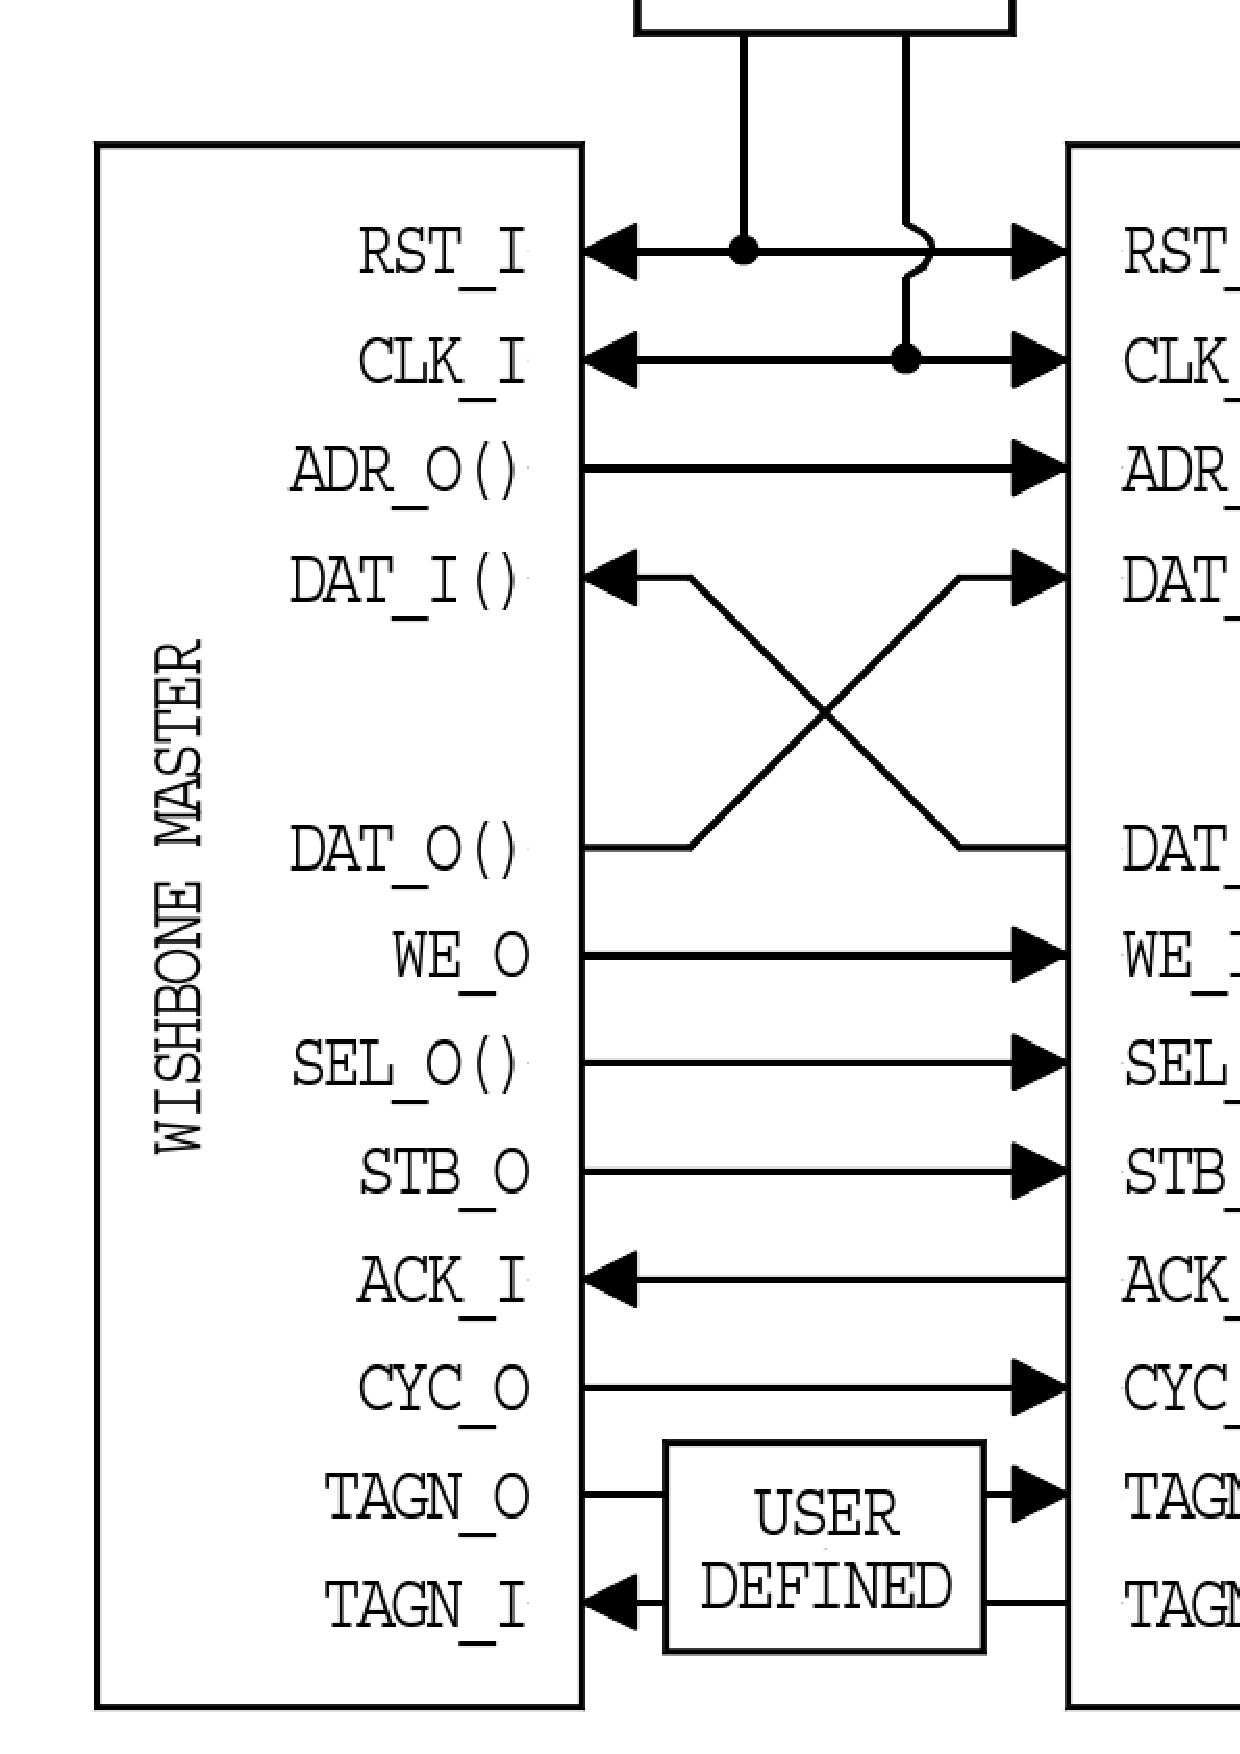
\includegraphics[width=8cm]{images/wishbone_bus.pdf}
% 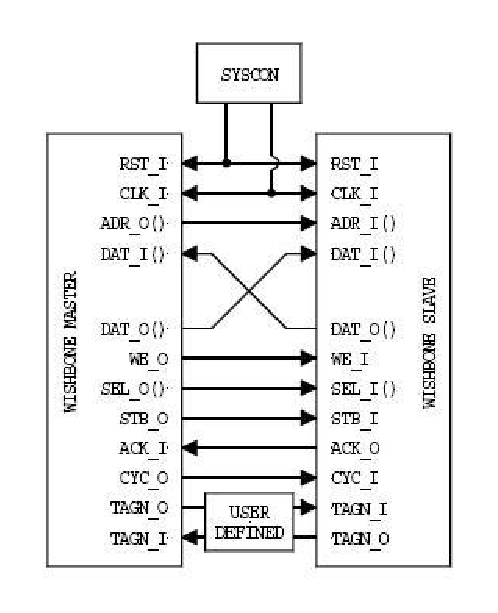
\includegraphics[width=8cm]{images/Wishbone_Bus_Point_to_Point.eps}
\caption[A Wishbone Point-to-Point Connection Scheme]{This is an example
implementation of a basic master-slave, point-to-point Wishbone interconnect.
The ``SYSCON'' design is not part of the Wishbone specification, it maybe
implemented however the designer sees fit.

Source: 'WISHBONE System-on-Chip (SoC)Interconnection Architecture for Portable
IP Cores', Revision: B.3, Released: September 7, 2002.}
\end{center}
\label{APP_Wishbone_P2P}
\end{figure}

\begin{figure}[h!]
\begin{center}
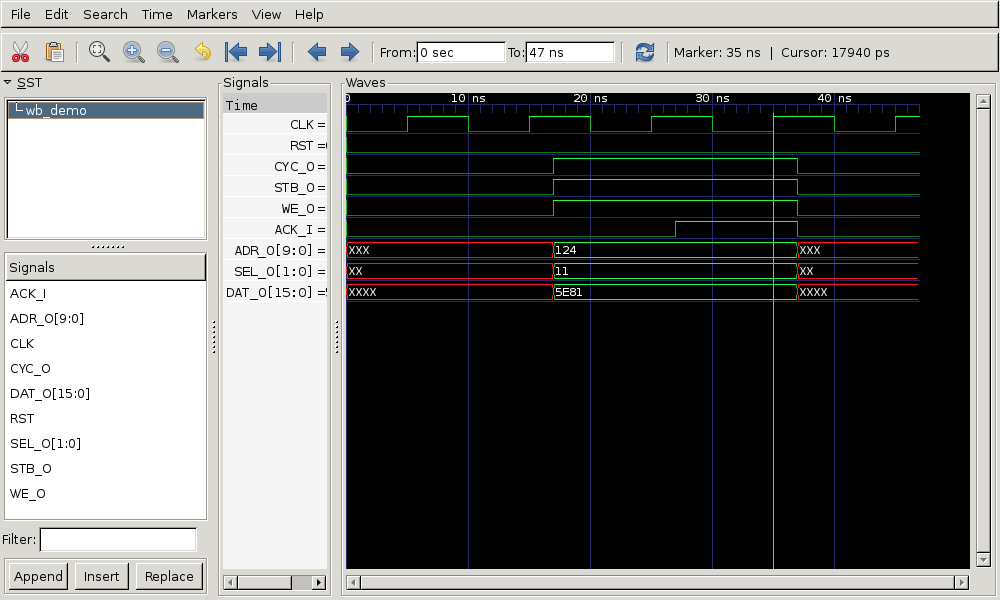
\includegraphics[width=\linewidth]{images/wishbone_demo.png}
\caption[A Sample Wishbone Transaction]{One 16-bit word is written by a master
to a slave device. The signals CYC$\_$O and STB$\_$O are asserted by the master to frame the transaction. The ACK$\_$I
response is received by the master and indicates that the slave has completed the
transfer.}
\end{center}
\label{APP_Wishbone_Sig}
\end{figure}


\section{Description of Wishbone Signals}
This section gives a brief summary of the main Wishbone signals. User-defined
tags were not used for OpenVGA's internal bus so these signals are not described.
Additionally, Wishbone bus ports to HDL modules used within OpenVGA include both
a prefix and a suffix. For example, the prefix ``wb'' of signal
``wb$\_$cyc$\_$o'' indicates that the signal is a Wishbone signal, and the
suffix ``o'' indicates that this is an output. (The output direction of the CYC signal would also
indicate that the module this signal belongs to is a Wishbone master.)

\begin{itemize}
  \item CYC: This signal is asserted by a master and it claims ownership of the
  Wishbone bus. Other masters on a bus are prevented from asserting their CYC
  when a CYC is already asserted. This signal is still used for non-bus
  topologies, like point-to-point, and is used in combination with STB to select a slave
  device.
  \item STB: This signal is asserted by a master and frames a Wishbone
  transaction. If a slave device has its STB input signal asserted, then it has
  been selected for a Wishbone transaction.
  \item WE: This signal is driven by a master and selects whether the
  requested transaction is a write or a read (signal levels high and low
  respectively).
  \item ACK: This signal is asserted by a slave to indicate that it has either
  received data, if the transaction is a write, or has placed valid byte
  selects and data on its data outputs, for a read transaction. This signal is
  asserted just once for each data transfer, and can take many cycles to assert, depending on the
  latency of the device.
  \item RTY: This signal is asserted by a slave to indicate that the device is
  currently unable to fulfil the current Wishbone request, and to retry
  later.
  \item ERR: This signal is asserted by a slave to indicate that an error has
  occurred. Wishbone does not specify how errors are handled except that the
  slave must leave the bus in a usable state at the end of the transaction.
  \item CTI[2:0]: This signal array is driven by the master and can request a
  burst transfer. Even if the master specifies a burst mode, the slave is not
  required to perform a burst transfer. Also, if the slave supports burst
  transfers but not the mode requested, it responds with single transfers. It
  is optional to implement this signal, it has to be set to zero for a slave
  that supports this signal when a master does not. A full description of the
  modes is available in the Wishbone specification\cite{WB3_Spec}.
 \item BTE[1:0]: This signal array is driven by the master and specifies the
 Burst Type Extension. This signal can only be implemented if CTI
 is also implemented, and is required to be implemented if CTI is implemented
 and the device supports burst transfers. A full description of the modes
 is available in the Wishbone specification\cite{WB3_Spec}.
 \item ADR: This signal array is driven by the master and is the
 address of the data requested for the transaction. This signal is
 optional, and its width is device dependent, a FIFO may not need an address,
 for example.
 \item SEL$\_$O[$n$-1:0] \& SEL$\_$I[$n$-1:0]: These signal arrays are driven
 by both masters and slaves and are used to select valid bytes within a data
 word. A 64-bit transfer has eight select bits, so $n=8$, for example. During a
 write transaction, the master asserts the valid bytes on its own SEL$\_$O
 outputs, and during a read transaction, the slave asserts the byte-valid
 selects on its SEL$\_$O outputs. A device that supports reads and writes is
 required to implement both SEL$\_$O and SEL$\_$I. These signals have to
 be valid when the device responsible for driving them has its STB or
 ACK signals asserted.
 \item DAT$\_$O[$m-1$:0] \& DAT$\_$[m-1:0]: These signal arrays are driven by
 both masters and slaves and are used to transfer data across the Wishbone
 interconnect. The width, $m$, must be one of 8, 16, 32, or 64. A master
 performing a write must have valid write data on its DAT$\_$O signals whenever
 its STB signal is asserted. A slave responding to a read request must have valid
 data on its DAT$\_$O outputs when its ACK signal is asserted. For
 point-to-point applications the DAT$\_$O of a device is typically connected to
 the DAT$\_$I of the other device.
\end{itemize}

All wishbone control signals are active when high (or ``1'') and
Figure~\ref{APP_Wishbone_Sig} shows an example transfer using many of the
signals described above.
